\begin{figure}[t]
\centering
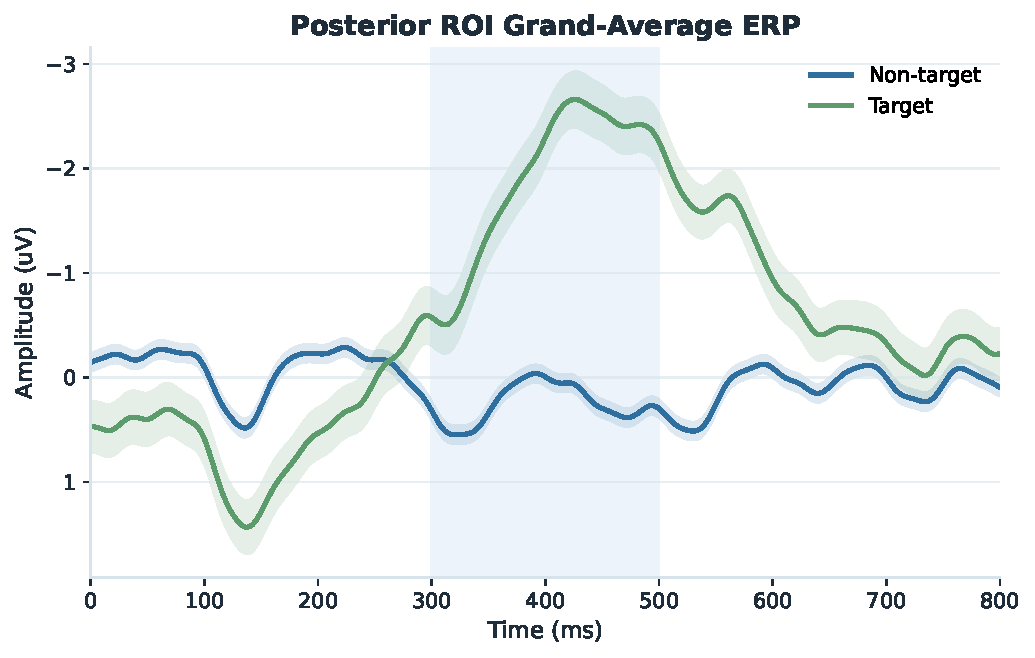
\includegraphics[width=0.92\linewidth]{figures/erp_grand_average_roi}
\caption{Grand-average posterior-region ERP waveforms for target and non-target trials, averaged across PO7, PO8, PO3, PO4, O1, and O2. Shaded bands denote the 95\% confidence interval across epochs, and the highlighted 300--500 ms region marks the canonical posterior P300 interval.}
\label{fig:erp_grand_average_roi}
\end{figure}

\begin{figure}[t]
\centering
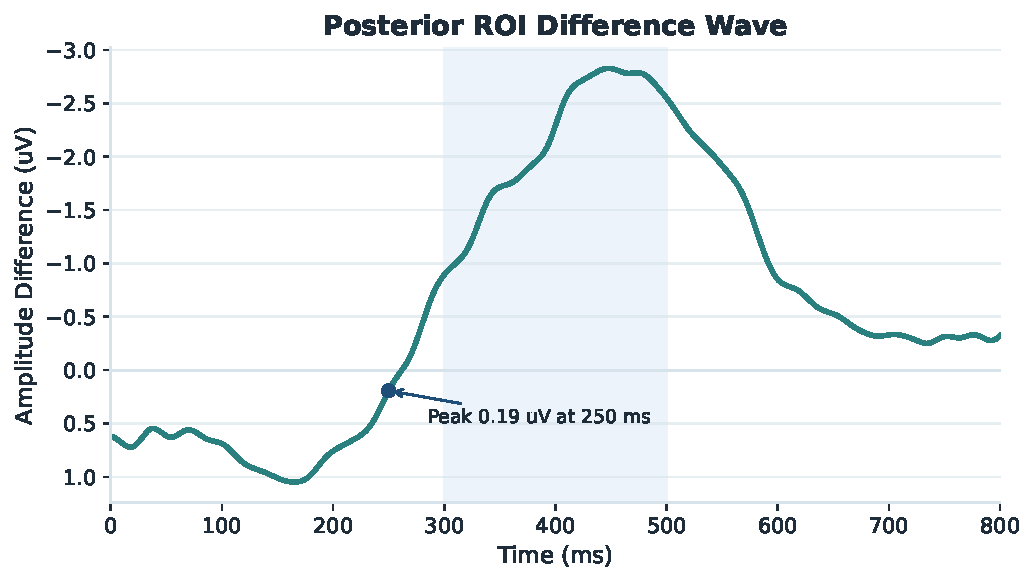
\includegraphics[width=0.92\linewidth]{figures/erp_difference_wave_roi}
\caption{Target-minus-non-target difference waveform for the posterior ROI. The annotated extremum was constrained to the target-related window and occurred at 400 ms with amplitude -2.30~$\mu$V, consistent with the strongest discriminative interval around 400-500 ms.}
\label{fig:erp_difference_wave_roi}
\end{figure}

\begin{figure}[t]
\centering
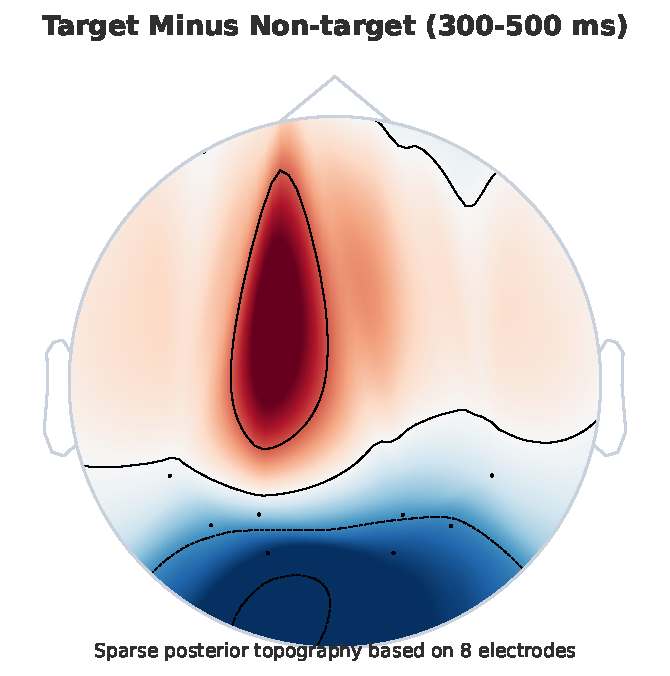
\includegraphics[width=0.72\linewidth]{figures/topomap_difference_300_500ms}
\caption{Sparse posterior scalp topography of the target-minus-non-target ERP amplitude averaged over 300--500 ms. Because the montage contains only eight electrodes, the map should be interpreted as a coarse posterior spatial summary rather than a dense reconstruction.}
\label{fig:topomap_difference_300_500ms}
\end{figure}

\begin{figure}[t]
\centering
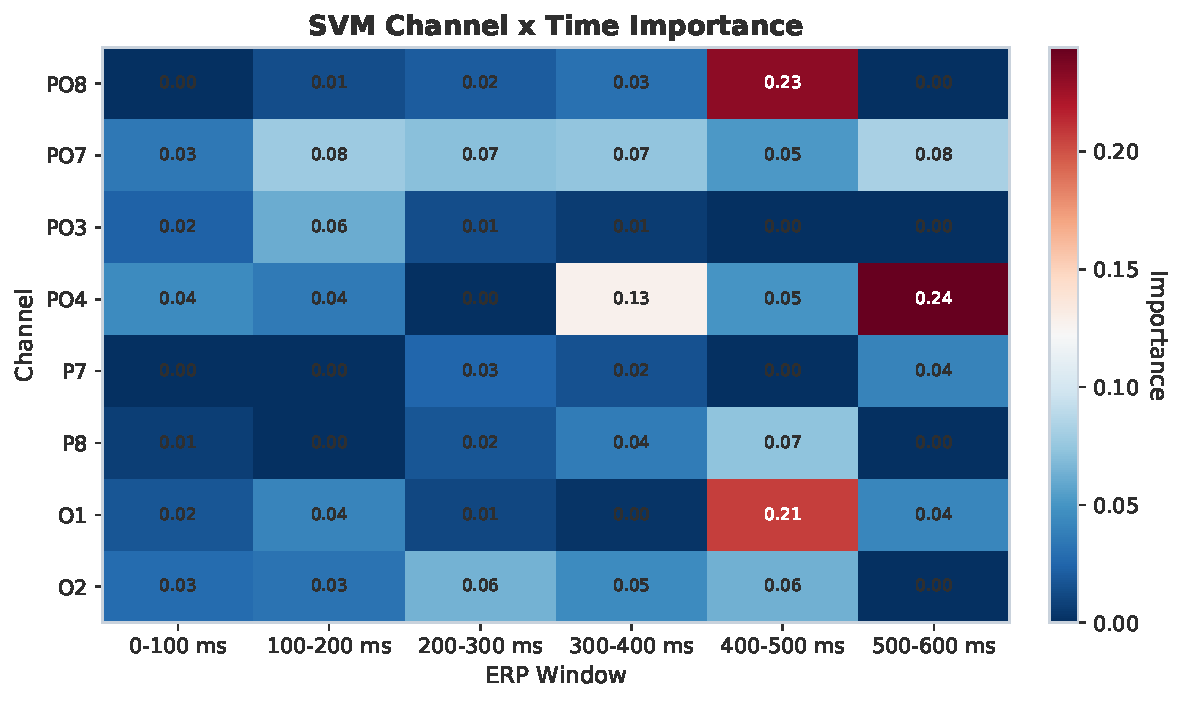
\includegraphics[width=0.98\linewidth]{figures/feature_heatmap_channel_time}
\caption{Channel-by-time-window importance heatmap for the best pooled classifier. The largest importance values cluster in the 400-500 ms interval and are concentrated over posterior channels, particularly PO4, PO7, O1.}
\label{fig:feature_heatmap_channel_time}
\end{figure}

\begin{figure}[t]
\centering
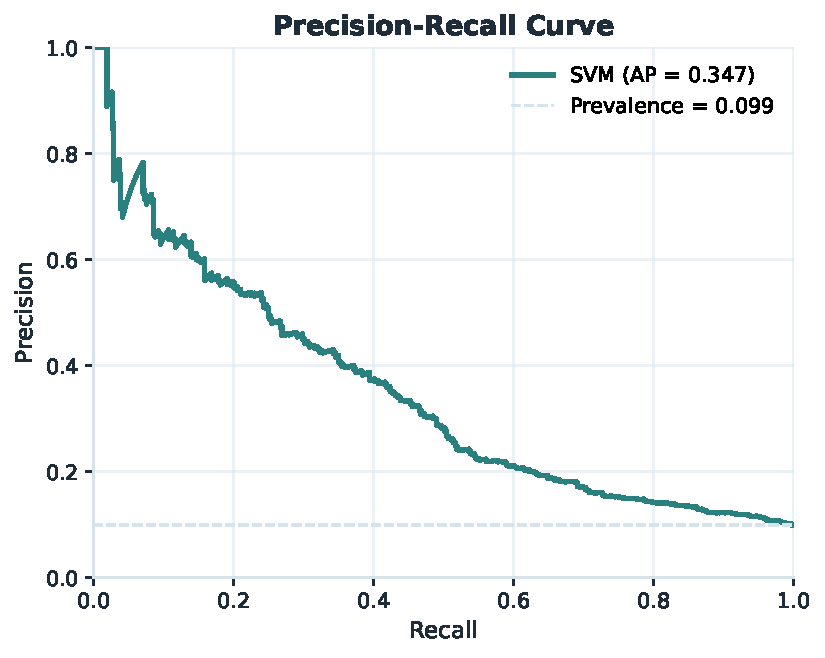
\includegraphics[width=0.82\linewidth]{figures/pr_curve_best_model}
\caption{Precision--recall curve for the best pooled classifier. The dashed horizontal line indicates the positive-class prevalence baseline, which is the appropriate reference under marked class imbalance.}
\label{fig:pr_curve_best_model}
\end{figure}

\begin{figure}[t]
\centering
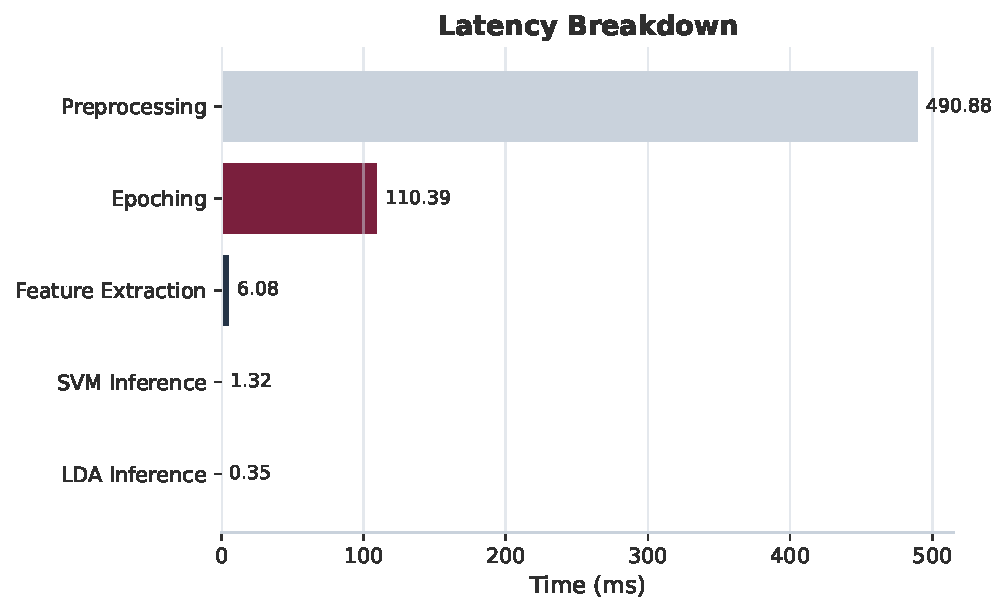
\includegraphics[width=0.90\linewidth]{figures/latency_breakdown}
\caption{Average latency of the main processing stages, including preprocessing, epoching, feature extraction, and single-sample inference, illustrating the computational cost of the lightweight ERP-based pipeline.}
\label{fig:latency_breakdown}
\end{figure}

Under the pooled random-split evaluation, the best-performing classifier was the SVM model, which achieved a balanced accuracy of 0.6729, recall of 0.5196, precision of 0.2480, F1 score of 0.3357, and PR AUC of 0.3467. The LDA baseline reached a balanced accuracy of 0.6771 with PR AUC 0.2960, whereas the class-weighted RBF-SVM achieved 0.6729 balanced accuracy and PR AUC 0.3467, indicating a modest but consistent advantage for a nonlinear decision boundary under marked class imbalance. The accompanying ERP-oriented interpretation localized the most informative features to the 400-500 ms interval and to posterior electrodes PO4, PO7, O1, in agreement with the target-related posterior ERP separation visible in the grand-average and difference-wave figures. Across the full processed dataset, the analysis included 2041 target epochs and 18493 non-target epochs, so the observed precision-recall trade-off should be interpreted as evidence that target-related information is detectable but still challenging to recover from a sparse eight-channel posterior montage in RSVP EEG.

The present results support the use of ERP-window features rather than spectral band-power summaries for RSVP attention detection, because the target-related signal in this paradigm is expected to be dominated by transient posterior ERP activity rather than sustained oscillatory changes. The importance analysis concentrated on the 400-500 ms interval and on posterior channels such as PO4, PO7, O1, which is neurophysiologically consistent with a P300-like target response over parieto-occipital scalp regions. The corrected posterior ROI difference wave also showed its annotated extremum within the target-related window rather than at the earliest boundary, which aligns the waveform interpretation with the channel-time importance summary and with the expected posterior P300 timing. At the same time, the moderate classification performance remains scientifically plausible given the strong class imbalance, sparse eight-channel montage, and cross-subject variability characteristic of rapid visual presentation datasets. These properties make the proposed approach valuable as a lightweight, explainable baseline that captures meaningful target-related ERP structure without relying on heavy preprocessing or opaque deep models.
